% !TEX root = mythesis.tex

%==============================================================================
\chapter{Theoretical Concepts and Experimental Basics}
\label{sec:SM}
%==============================================================================

\section{The Standard Model (SM)}

In the 19th century, John Dalton postulated that matter is made up of small indivisible 
pieces called atoms. Since then, technological advancements and human curiosity have empowered 
us to explore various phenomena around us in greater detail. Eventually, our understanding of nature 
evolved, leading to the development of the Standard Model of Particle Physics, which explains the 
fundamental structure of matter. Consisely speaking, the Standard Model (SM) of particle physics is a 
theory that explains almost everything that nature has to offer. It is based on fundamental particles 
and their interactions being governed by Quantum Field Theories (QFTs). The SM has precisely predicted
existence of various particles and their properties. Testing the SM and its predictions plays a
crucial role in deciding the physics program of Particle Physics experiments.  

The Standard Model is divided into spin-1 fermions and spin-0 bosons. The fermions are
further divided into leptons and quarks as shown in \cref{fig:SM}. Another
classification of fermions is into generations. The first generation constitutes
\Pup, \Pdown, \Pelectron and \Pnue which forms the surrounding matter. The second
and third generation particles are high energy \textit{siblings} of the first generation
particles. These are observed at high energies such as colliders. The SM also includes
anti-particles which are clones of particles with opposite quantum numbers.


\begin{figure}[htbp]
    \centering
    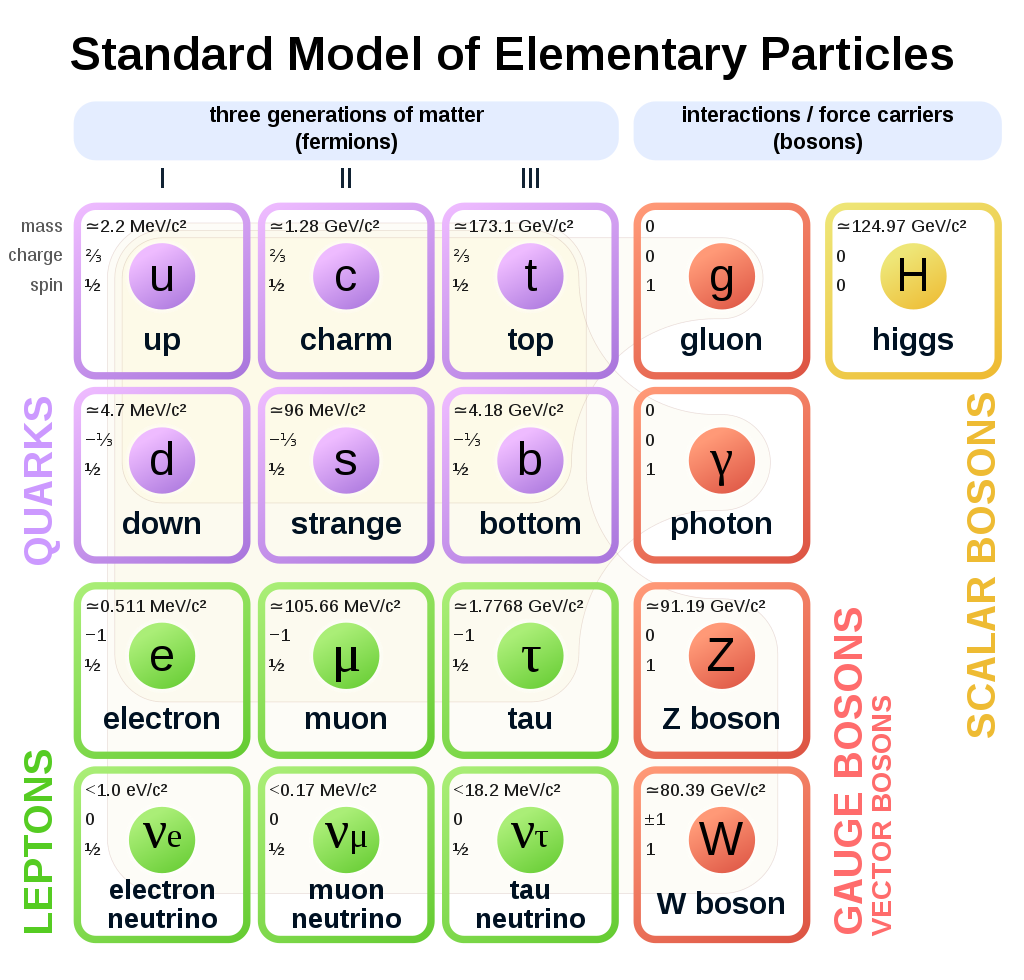
\includegraphics[width=1.1\figwidth]{SM.png}
    \caption[Standard Model of Particle Physics]{Overview of the particles in the Standard Model 
    along with their properties including mass, spin and charge are shown. Particles shown in lavender 
    and green are fermions while the ones shown in red are gauge bosons. The three generations
    are also highlighted by roman letters. Anti-particles are not shown~\cite{SM}.}%
    \label{fig:SM}
\end{figure}

These fermions interact with each other via exchanging bosons which are also called 
\textit{force-carrier} particles. The photon (\Pphoton), which is massless and carries no electric 
charge, is the messenger of the electromagnetic (EM) force, experienced only by charged particles.
The underlying QFT is called Quantum Electrodynamices (QED) based on the U(1) symmetry group. The more
commonly known electrostatic attraction between charged particles is the low-energy manifestation of QED. Among 
the SM, all fermions except neutrinos are sensitive to the EM force. The strength of the EM force
is expressed by its dimensionless coupling constant,

\begin{equation}
    \alpha \sim \frac{1}{137}
\end{equation}

The strong interaction, mediated by massless gluons, is experienced by particles 
carrying the so-called \textit{colour} charge. The physics behind the strong interaction is 
explained in Quantum Chromodynamics (QCD). The quarks, which are the only particles carrying colour charge,
can interact via the strong interaction. A peculiar thing in QCD is that the gluons themselves also 
carry colour charge. This property is unique for a force-carrier particle. 

The weak force carriers are the vector bosons, \PWpm and \PZ, which unlike \Pphoton and 
gluons, are massive and charged in case of \PWpm boson. The \PZ boson is electrically neutral. The weak
interaction manifests itself in phenomena such as $\beta$-decay and fusion processes inside the sun. All the
SM particles, including the neutrinos, are sensitive to the weak force. 
The interaction mediated by \PWpm and \PZ is called charged-current weak interaction and
neutral-current weak interaction, respectively. The famous Wu experiment~\cite{Wu:1957my} proved that 
the charged current weak interaction violates parity. The parity violating nature of the weak interaction
suggests that the interaction vertex must be different from that of QED and QCD. Studies showed that
the weak interaction is described using a $V-A$ vertex and this fact dictates that only left-handed
chiral particle states and right-handed chiral antiparticle states can participate in 
charged-current weak interaction. 

The theory unifying QED and the weak interaction is called the Electroweak theory explained in 
\cref{sec:ewtheory}. The last piece of the SM puzzle, which is the last discovered fundamental particle,
is the Higgs boson. It is a spin-0 boson, unlike other bosons. All particles acquire their mass 
through the Higgs mechanism.

\subsection{Feynman diagrams}

There are numerous probable interactions between SM particles and having a tool to visualise them
would greatly aid in understanding the underlying physics. In Particle Physics, a tool called Feynman
diagrams is used for this purpose. 

These diagrams are symbolic representations of particle interactions. They make use of straight lines 
with arrows to show incoming and outgoing particles and anti-particles. Wavy lines are used to show
the boson exchanged between them. It also has a hypothetical time axis which demonstrates the
evolution of the process with time. The Feynman diagrams are just a pictorial representation and have no 
physical meaning. 

Consider an example of electron-position scattering (also known as Bhabha scattering). In the Feynman diagram,
shown in \cref{fig:bhabha}, let's suppose a horizontal time axis. The diagram reads as following:
an electron and positron enter, a photon is exchanged between them and the two particles exit. The point of
interaction between two particles is called a \textit{vertex}.
It is important to note the direction of arrows in particle lines. The arrow directions are opposite 
for particles and antiparticles. 
In the shown diagram, the incoming electron points in the forward direction, denoting the 
evolution of the interaction with time, whereas the incoming positron points in the backward direction.
It can be seen that the arrow directions together represent the continuous current flow. 


\begin{figure}[htbp]
    \centering
    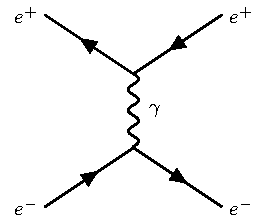
\includegraphics[width=0.6\figwidth]{bhabha-tikz.pdf}
    \caption[Sketch of the ATLAS calorimeters]{A Feynman diagram showing the Bhabha scattering}%
    \label{fig:bhabha}
\end{figure}

The quantitative analysis for a process includes two important steps: accessing the Feynman diagrams to
compute the amplitude ($\mathcal{M}$) and together with the phase space, calculating quantities such as 
decay rate, cross-section and differential cross-section. The Feynman diagrams are 
analysed through a set of rules called Feynman rules. It is important to note that
for each process, there are infinite possible Feynman diagrams which require to be summed to get the 
accurate final process description. The diagram shown in \cref{fig:bhabha} is a basic diagram with particles 
entering and exiting, called real particles with specific masses. A
process can also have intermediate stages where off-shell intermediate particles
with varying masses, called \textit{virtual} particles are produced. Presence of intermediate states lead to 
more vertices inside a diagram and therefore give rise to a plethora of Feynman diagrams for a certain 
process. 

In the context of Feynman calculus, each vertex within a diagram contributes a factor equal to the 
coupling constant of the interaction. Hence, the actual process can be quantitatively described in terms
of expansion with respect to the coupling constant. For the expansion to converge, the coupling constant
needs to be small. The most basic diagram with the lowest order expansion
is called "tree-level" or "leading-order (LO)" diagram. The diagram corresponding to the next order
of expansion is called next-to-leading-order (NLO). Higher order diagrams with more vertices 
contribute less owing to the small couping constant. 


\subsection{The Strong Force}
Electrons and nucleus inside an atom are held together by the electromagnetic force. The same 
force also exists between protons inside the nucleus causing repulsion. However, there exists a force
which is strong enough to overcome repulsion and keep the nucleus together. It is called the strong force or 
the strong nuclear force. The QFT describing the strong force is called Quantum Chromodynamics (QCD) and the
underlying symmetry group is SU(3) described by $3 \times 3$ matrices. The eight generators of the SU(3) group
give rise to eight gluons which are the strong force mediators. The structure of the SU(3) group demands that 
the wave function of the strongly interacting particle must be a 3-component vector. This gives rise to 
a new degree of freedom called "colour", with three states called red, blue and green. Consequently, particles
having a non-zero colour charge can feel the strong force. Among the SM particles, only quarks have the colour
charge which can be either red, blue or green.

A major differentiating factor between QCD and QED is that the gauge boson in QCD carries the charge of 
interaction. In other words, gluons also carry the colour charge which allows them to interact with other 
gluons as well. As a result of this self-interaction, no coloured object can be found as a free particle in 
nature. Due to this so-called colour confinement, quarks cannot exist independently but instead are found in
colour-neutral states called \textit{hadrons}. For instance, if two quarks are pulled away from each other, a gluon field is 
created between them which is proportional to the separation. The gluon fields is so strong that at some point,
the energy in this field is sufficient to produce new quarks and antiquarks that form colourless bound states.
This process is called hadronisation. Due to colour confinement, only certain configurations for hadrons
are permitted. The possible combinations discovered so far can be categorised into mesons (\Pquark\APquark),
baryons (\Pquark\Pquark\Pquark) and antibaryons (\APquark\APquark\APquark).

The value of the strong coupling constant, $\alpha_S$, is relatively larger than the coupling 
constant of QED. As a consequence, contribution of higher order Feynman diagrams
increases and it becomes difficult to implement perturbation theory for QCD calculations. One of the
great discoveries in QCD is that the strong coupling constant is in fact not a "constant" but instead the
value is dependent on the energy scale of the interaction~\cite{Deur:2016tte}. The running of $\alpha_S$ means that at low
energies, the force between the quarks is stronger (larger $\alpha_S$) whereas at higher energies, the 
force becomes weak (smaller $\alpha_S$). The running of $\alpha_S$ allows us to apply perturbation theory
at high energies and this property is called asymptotic freedom. 

\subsection{The Electroweak theory}
\label{sec:ewtheory}
In the 1960s, physicists were trying to formulate a gauge theory for weak interactions
similar to QED. A theory can be a gauge theory if it has an underlying mathematical symmetry
and it is renormalisable. A quantum field theory is renormalisable if the divergences can be absorbed
by implementing finite number of parameters, such as, coupling constant. Glashow,
Salam and Weinberg discovered such a gauge theory by unifying electromagnetic force and 
the weak force.

The electroweak (EW) theory is a unification of QED and the thoery of weak interactions. 
It is described by the symmetry group $SU(2)_L \otimes U(1)_Y$. The corresponding
charges of the electroweak theory are the weak isospin $I,I_3$ and the weak hypercharge $Y$.
The weak hypercharge $Y$ determines the interaction under the $U(1)$ transformations.
The weak isospin of particles determines their transformation under $SU(2)$ and therefore, it is
used to make multiplets of particles. The left-handed leptons ($\Plepton_L$) will form doublets
because they transform into each other under the influence of weak force. 
This is due to the $V-A$ vertex form of the weak interaction. On the other hand, the right-handed 
particles are singlets ($\Plepton_R$). 

\begin{align}
    \Plepton_R = e^{-}_R, \mu^{-}_R, \tau^{-}_R \\
    % \Plepton_R = \Pelectron_R, \Pmuon_R, \Ptau_R \\
    \Plepton_L = \begin{pmatrix} \Pnue \\ \Pelectron \end{pmatrix}_L , \begin{pmatrix} \Pnum \\ \Pmuon \end{pmatrix}_L , \begin{pmatrix} \Pnut \\ \Ptau \end{pmatrix}_L 
\end{align}

The Lagrangian of the EW model introduces three bosons $\PW_\mu^{(1,2,3)}$ corresponding
to $SU(2)$ and one $B_\mu$ corresponding to $U(1)$. Th experimentally observed $\PWpm$
are combination of $\PW_\mu^{(1)}$ and $\PW_\mu^{(2)}$ whereas photon ($A$) and the Z-boson are linear
combinations of $\PW_\mu^{(3)}$ and $B_\mu$ based on the weak mixing angle ($\theta_W$)
as given below:

\begin{align}
A_\mu = +B_\mu \text{cos} \theta_W + W_\mu^{(3)}\text{sin} \theta_W \\
Z_\mu = -B_\mu \text{sin} \theta_W + W_\mu^{(3)}\text{cos} \theta_W 
\end{align}

The weak interaction for the quark sector can be explained by creating similar
$SU(2)$ doublets(Q).

\begin{align}
    Q = \begin{pmatrix} u \\ d' \end{pmatrix}, \begin{pmatrix} c \\ s' \end{pmatrix}, \begin{pmatrix} t \\ b' \end{pmatrix}
\end{align}

The strength of the weak interactions for quarks is determined experimentally by studying
nuclear $\beta$-decay. It is observed that the vertices corresponding to different quark
flavours have different coupling strengths. The reason for this is given by the Cabibo
hypothesis which states that, the flavour eigen states that participate in the weak interactions
are a mixture of the mass eigen states. The relation between them is given by the 
Cabibo-Kobayashi-Maskawa (CKM) matrix. 

\begin{align}
    \begin{pmatrix} d' \\ s' \\ b'\end{pmatrix}
     = \begin{pmatrix} V_{ud} & V_{us} & V_{ub} \\
                       V_{cd} & V_{cs} & V_{cb} \\
                       V_{td} & V_{ts} & V_{tb}
    \end{pmatrix} \begin{pmatrix} d \\ s \\ b\end{pmatrix}
\end{align}

The values of the CKM matrix elements can be found in \cite{pdg2024}. The diagonal
of the matrix is close to unity, suggesting that the weak interaction is stronger within
the same generation of quarks. 

The experiments at the Gargamelle bubble chamber in 1973 hinted the evidence of a neutral
massive boson responsible for the observed neutrino interactions~\cite{HASERT1973138}. In 1983, the \PZ-boson
was directly discovered at the Super-Proton Synchrotron at CERN. The electroweak theory
was verified by this pathbreaking discovery. The properties of the \PZ-boson were
studied at the Large Electron-Positron (LEP) collider at CERN. The discovery of \PZ and \PW 
bosons are among the crucial tests of the Standard Model. 


\subsection{The Higgs mechanism}
According to the electroweak theory, weak bosons are required to be massless for the 
underlying symmetry to be preserved. However, experiments revealed that the weak gauge bosons, \PW and 
\PZ have finite masses~\cite{Brout-Englert-Higgs:1998492}. The explanation of this spontaneous symmetry breaking was given by the 
Brout-Englert-Higgs mechanism~\cite{PhysRevLett.13.508}.
Particles in the SM acquire their mass through the Higgs mechanism. It is a way of 
spontaneously breaking SM symmetries by introducing a new field called the Higgs field. The strength of
interaction of particles with this field determines how massive the particles will be. Higgs mechanism
implies the existence of a scalar particle, the SM Higgs boson. In a landmark discovery, the Higgs 
boson was independently discovered by ATLAS and CMS in 2012~\cite{ATLAS:2012yve,CMS:2012qbp}. Since then,
the Higgs boson studies are an important part of the LHC physics program. 

\section{Limitations of the SM}
The Standard Model is a highly successful theory that has been tested at various collider experiments 
and almost all the experimental results agree with the predictions, at a high degree of precision. Despite
its enormous success, there are still some drawbacks of the SM. They are summarised below:

\begin{itemize}
    \item Out of the four fundamental forces, only three are explained in the SM. Gravity is not included.
    \item SM predicts that neutrinos are massless but experiments have proved that neutrinos are not massless.
    \item The difference in the mass scale of vector bosons/Higgs boson and the Plank scale is extremely 
    large. This is known as the hierarchy problem and is unexplained by the SM.
    \item There is no explanation of why is there more matter around us than antimatter.
    \item The possible existence of dark energy and dark matter is hinted from studies regarding
    expansion of the universe. There is no explanation in the SM. 
\end{itemize}

\section{Physics at the hadron colliders}

% \subsection*{Natural units}

\subsection*{Center-of-mass energy}
In a collision between two particles the total center-of-mass energy is expressed as
\begin{equation}
    \sqrt{s} = \sqrt{(\Sigma_{i = 1}^{2} E_i)^2 - (\Sigma_{i = 1}^{2} p_i)^2},
\end{equation}
where $E$ and $p$ are energy and momentum of the two initial state particles. If two colliding beams 
of the same particle type have the same energy, then the center-of-mass energy is 
$\sqrt{s}$ = $2E_{beam}$, neglecting the masses of particles. 

\subsection*{Decay rate and branching ratio}

An elementary particle often decays into smaller particles through the possible decay modes or 
channels, depending on the conservation laws for quantum numbers and strength of the decay process. 
The probability per unit time of a particle decaying is called its decay rate ($\Gamma$). For $N$ 
identical particles the change in the number after time \textit{dt} is given by
\begin{equation}
    dN = - \Gamma N dt.
\end{equation}

The lifetime of the particle is the time after which the sample becomes $\frac{1}{e}$ of its original 
size,
\begin{equation}
    \tau = \frac{1}{\Gamma}.
\end{equation}

When multiple decay modes are possible, the total decay rate of the particle is the sum of individual 
decay rates. In order to learn the dominance of a certain decay mode, we calculate its branching 
ratio (BR). The branching ratio of a decay mode $i$ is defined as
\begin{equation}
    \text{BR} = \frac{\Gamma_i}{\Gamma_{\text{total}}}.
\end{equation}


\subsection*{Parton Distribution Functions (PDFs)}
Protons at the LHC collide at high energies giving rise to deep inelastic interactions called hard processes.
In such cases, the interactions are not between protons but between their constituents which are
quarks and gluons, collectively known as \textit{partons}. These partons carry a fraction of the total
momentum of the proton (or a hadron in general). In order to study an interaction, it is important to
know the effective energy of the interacting partons and their flavour. This information is encoded in 
the Parton Distribution Functions (PDFs). It describes the probability of finding a parton of 
certain flavour $i$, carrying a momentum fraction $x_i$ at a certain energy scale.

\subsection*{Pileup}

IMAGE OF PILEUP PROFILE RUN2

The 
primary hard scatter collisions, that are of interest, are contaminated by soft interactions 
called pileup. It is defined by the average number of interactions
recorded per bunch crossing. Sources of pileup are categorized into in-time and out-of-time pileup. In-time pile up is due to collisions
occurring in the same bunch-crossing and out-of-time pile-up is contributed by the collisions from previous
or later bunches. Some of the sub-detectors have sensitivity windows longer than the interval between
bunch crossings. This eventually affects the recorded number of interactions per bunch. The accurate
detection of objects under study becomes difficult due to pile-up events. The higher the 
luminosity, more the pileup. The object reconstruction algorithms have dedicated procedures 
to mitigate pileup.

\subsection*{Luminosity and cross-section ($\sigma$)}
The quantity that measures the ability of a collider to produce particle interactions is called
instantaneous luminosity ($\mathcal{L}$). The instantaneous luminosity integrated over the lifetime
of collider operation is called integrated luminosity ($L$).

In order to define the event rate for interesting processes, along with luminosity, we require
another quantity called the cross-section. At the subatomic scale, the particle interactions 
are governed by the laws of quantum physics. Therefore, a theory can predict 
the \textit{probablility} of certain outcomes of collisions. The probability of a certain
process to occur is called its cross-section ($\sigma$). Finally, the number of event rate of
specific interactions is defined as the product of integrated luminosity and the cross-section (\cref{eq:lumi}).
\begin{equation}
    R = \sigma \cdot \int_{dt} \mathcal{L}(t)
    \label{eq:lumi}
\end{equation}

For a particle collider, beam energies and the luminosity are two important figures of merit. 
High energy allows the production of new heavy particles and high luminosity allows more flux 
of particles contributing to high number of collisions.

\subsection*{Differential cross-section}
Differential cross-section is a type of cross-section which gives the probability of an interaction
with respect to a variable X. In common practice, differential cross-section is defined as $d\sigma/dX$,
where $dX$ can be solid angle in scattering experiments or kinematic variables such as \pT. The 
integral over the entire range of $X$ gives the total cross-section. 

The differential cross-section offers a deeper insight into the process of interest. For example, in a 
scattering experiment designed to investigate the internal structure of a target, the scattering 
profile of the incident particles is analysed. If the scattering rate varies at different solid angles,
 this variation will be captured in the differential cross-section measurements. 

Another advantage of studying differential cross-section is that if there is any new physics,
it may manifest itself by altering the kinematic distributions of known SM particles. Measuring the 
differential cross-sections with respect to kinematic variables and then comparing them to SM predictions
is one of the crucial tests of the SM. Any deviations in the comparison can hint towards new physics.
A differential analysis is based on the shape of the kinematic distribution and not just the 
total events in the distribution. Therefore, differential cross-sections can be used for various
theory interpretations.

\section{Top quark physics}
The top quark was discovered in 1995 at the Tevatron laboratory(?) by the CDF collaboration[CITE].
It is the heaviest fundamental particle discovered so far with a mass of \SI{173}{\GeV}[CITE PDG] 
and since it is close to the EW scale, the top quark might play an important role in understanding
Electroweak Symmetry Breaking (EWSB). Moreover, the fact that $m_t$ is greater than $m_H$ hints whether
the top quark gets its mass through Higgs mechanism.  

The top quark is the weak isospin partner of the bottom quark and thus completes the three 
generation structure of the SM. Since its discovery, top quark has been a crucial part of
any physics program at the hadron colliders because of its heavy mass. It decays almost exclusively
into W and b before hadronisation. This property gives us a unique opportunity to study a "bare"
quark because some top quark properties are conserved in the decay process and passed on to 
its decay products.

The LHC is a top factory becuase it can produce abundant top quarks and other related processes.
Therefore, LHC provides a lot of data which is analysed extensively to understand the top quark and
its properties. The production of top quarks is mainly through three kinds of processes: Wt-channel,
t-channel and the s-channel.









